\newpage
\section{Threads}
\subsection{Description}
\subsubsection{Thread Control Block}
A thread is represented in the memory by the \textbf{Thread Control Block}, a structure that contains all the relevant information like:
\begin{itemize}
	\item Thread \textbf{characteristics}: thread ID, name of the program
	\item \textbf{State information}: instruction counter, stack pointer, register contents
	\item \textbf{Management} data: priority, rights, statistics
\end{itemize}
\subsubsection{Management}
Big systems can have thousands of threads, therefore we need efficient ways to manage them. There are different options:
\begin{enumerate}
	\item Single threads not connected to each other
	\item All the threads are in a static long array
	\item All the threads are in a linked list of  variable length
	\item Tree
	\item The threads are managed via an inverted table
\end{enumerate}
In general, to increase \textbf{efficiency}, threads that forms a subset regarding a particular attribute (e.g. thread state) should be grouped together.
\subsubsection{Static and dynamic OS}
Depending on the OS type, threads may be managed differently:
\begin{itemize}
	\item \textbf{Static OS}: all threads (one per application) are statically defined in advance and the TCBs are declared as variables.
	\item \textbf{Dynamic OS}: the threads are created and deleted by kernel operations
\end{itemize}

\subsubsection{Address Space}
A logical address space of a thread is the set of its valid addresses that it can access. Modern CPUs allow \textbf{relative addressing} and address translation via a Memory Management Unit. This allows to have an arbitrary number of logical addresses mapped to a physical address space.\\
This also leads to mutual protection since the address spaces are \textbf{independent}, while at the same time allowing \textbf{relations}:
\begin{itemize}
	\item  A thread owns one \textbf{private address} space (Unix process)
	\item Several threads \textbf{share} an address space (Thread)
	\item A thread \textbf{switches} from an address space to another
\end{itemize}

\subsection{Switch}
Thread switching means that the processor stops the execution of the current thread and continues with the execution of another. It's the transition from one instruction sequence to another.
\subsubsection{Jumping}
Switching by jumping means using a \textit{jump} instruction (programmed statically) to jump to another thread. A switching point consists of:
\begin{itemize}
	\item \textbf{Continuation address}: where we interrupted the work
	\item \textbf{Jump instruction}
\end{itemize} 
The only use case for this type of approach is for very specific real time applications, to reduce as much as possible the latency. At the same time it's very \textbf{inflexible} since we often don't know from where we return , which one is the next thread and we often need the values of the registers.

\subsubsection{Context switch}
\paragraph{Continuation address} The first phase is to store the address of the next instruction to be executed in a special variable \textbf{ni}, located in the TCB.
\paragraph{Selection of next thread} The next thread to be executed is often determined at the moment of the switching, following different criteria:
\begin{itemize}
	\item \textbf{Cycling switching}: number of thread
	\item Order of arrival
	\item \textbf{Priority}: in this case the order can be organized in two dimensions, where each row is a group of threads with the same priority. It can be: 
	\begin{itemize}
		\item Constant
		\item Dynamic
	\end{itemize}
\end{itemize}
The selection problem can be solved inserting the threads in the selected order at the arrival.

\paragraph{Context switching} The \textit{jump} switch loses the content of the registers. In this case, we save the \textbf{state of execution} (arithmetic registers, index registers, processor state, etc..) and the \textbf{thread execution environment} (address registers, segment tables, interrupt masks, etc..) as a \textbf{thread context}.\\
This is the most consuming part of the switch, therefore there are special instructions and registers to speed up the process

\begin{observation}[Subroutine]
	To avoid redundant calls, we can use the switch as a common \textbf{subroutine}. In this way, when a thread calls for the switch, the second thread can come back directly to the same subroutine avoiding the save of the \textit{continuation address}.
\end{observation}

\begin{observation}[Thread control]
	Assuming the paradigm of \textbf{cooperative scheduling}, when the first thread calls for the switch subroutine, both the caller and the next thread need to give up and get the control at the same time. This is done by changing \textbf{stack pointer}.
\end{observation}

\subsection{Conditioned switching}
When a thread needs to wait for something to happen, the processor could do some other work instead of waiting. Therefore this happens when a certain condition is met.

\subsubsection{Thread states}
When a thread is waiting and we choose to switch to another one, we may encounter a thread that's also waiting and so on. To speed up the search for a working thread we divide them by \textbf{states}:
\begin{itemize}
	\item \textbf{Running}: threads that are currently being executed
	\item \textbf{Ready}: threads that are ready to be executed and are waiting for the processor
	\item \textbf{Waiting}: threads that are blocked and waiting for some external event
\end{itemize}
We handle state changes via these transitions:
\begin{itemize}
	\item \textbf{Relinquish}: voluntarily switching to another thread
	\item \textbf{Assign}: taking the next thread from the ready set to resume its operation on the processor
	\item \textbf{Block}: leave the processor since the condition is not met and must not be resumed until then
	\item \textbf{Deblock}: if the event happened for which the blocked thread waited it changes its state from waiting to ready and is inserted into the set of ready threads
\end{itemize}
\begin{center}
	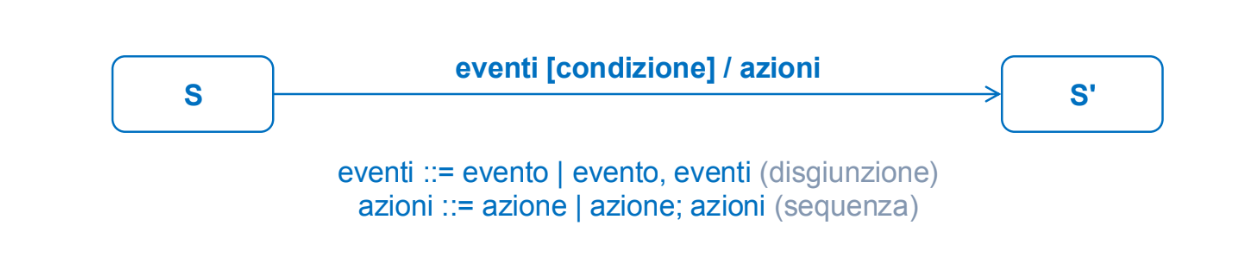
\includegraphics[scale=0.3]{transitions.png}
\end{center}

\begin{note}
	State change operations may also include other actions such as a thread switch. E.g. for the \textit{relinquish}.
\end{note}

\subsection{Automatic switching}
In many cases it's not viable to insert a switch call inside the thread. In this case we need an automatic way of doing that through a \textbf{clock} that specifies:
\begin{itemize}
	\item The deadline for each thread, called a \textbf{time slice}
	\item Interrupt on timeout
\end{itemize}
Since in this case it's the kernel that handles the switch, it needs to save the stack pointer, the interrupt pointer and the flags of the current thread to its own stack. Doing so, it can be pushed back again when it's his turn.

\subsubsection{Kernel exclusion}
When working with automatic switching we need to make sure that during the switch no other kernel operations are done, since they all work on the same shared data structures. This could cause faulty behaviors, e.g. during a condition evaluation a switch occurs.\\
To avoid this we use \textbf{mutual exclusion}, and in the case of the kernel we handle it entirely as a \textbf{critical section}. We distinguish four cases:
\begin{itemize}
	\item Single processor with no interrupts: we don't have problems
	\item Single processor with interrupts: we disable interrupts during kernel operations
	\item Multi processor with no interrupts: we use a \textbf{spin lock}, called also \textbf{busy waiting}, where we constantly check if the kernel is busy
	\item Multi processor with interrupts: we disable the interrupts and then we check if the kernel is lock, if that's true we enable them and stay in busy waiting. Otherwise we do the kernel operation and then enable them.
\end{itemize}

\subsection{Dynamic system}
In these types of systems the number of threads is variable. Therefore we need the following operations:
\begin{itemize}
	\item \textbf{Activate/Deactivate}: a thread exists (there is a TCB) but it's "resting". We use these operations to change from the state \textit{active} and \textit{inactive}
	\item \textbf{Create/Delete}: if the thread does not exist we need to create and then delete them
\end{itemize}
\begin{center}
	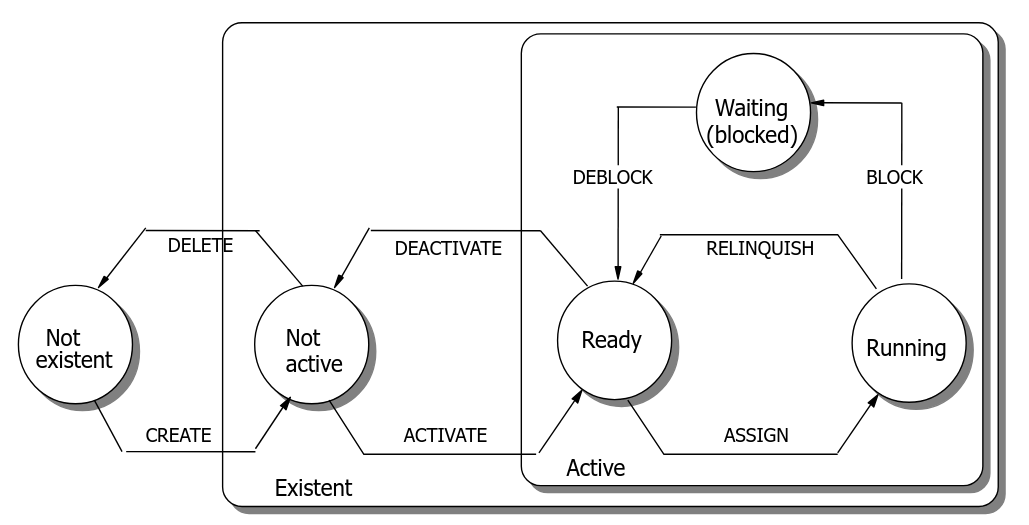
\includegraphics[scale=0.4]{state_diagram.png}
\end{center}

\subsubsection{Preemption}
There may be thread whose execution is really urgent and that cannot wait for a switch to happen. When these threads show up, the switch happens immediately and the first one is being \textbf{preempted} by the one with the higher priority. \\
In practice, we check for preemption whenever a new thread is added to the queue.

\subsubsection{Idle}
In operating systems with waiting states it may happen that all threads all waiting for something. To handle this we add an \textbf{idle thread} that:
\begin{itemize}
	\item \textbf{Never stops}
	\item has the \textbf{lowest priority}
	\item must be \textbf{preemptable} at any time
\end{itemize}
In practice we could use an empty loop (but wastes energy), a special operation like \textit{halt} that does not access memory but reacts to external signals, or a thread that does useful operations like checks and reorganizations.

\subsubsection{Initialization}
To switch to a thread for the first time we use the \textit{switch} procedure. To do so we need to prepare the TCB and the Stack as if it was already in the middle of a switch.

\subsection{Programming languages}
Many modern programming languages contain a thread concept to formulate concurrent activities within programs (e.g. Java Threads), or there are programming libraries that extend it by a thread concept. In these cases the threads are invisible to the OS, which sees the whole program as a thread.